%\documentclass[fleqn]{book}
\documentclass[11pt]{amsbook}

\usepackage[turkish]{babel}

%\usepackage{../HBSuerDemir}	% ------------------------
\usepackage{../Ceyhun}	% ------------------------
\usepackage{../amsTurkish}


\begin{document}
% ++++++++++++++++++++++++++++++++++++++
\hPage{ceyhun-188}
% ++++++++++++++++++++++++++++++++++++++

\footnote{"Tanım 4.1.4" should have been written, yet I could not find the tag label any of the templates.} Çizgedeki bir ayrıtın, dizi bağlı iki ayrıtla değiştirilmesine, \textit{\underline{dizisel değiştirim işlemi}} denir.

\footnote{"Tanım 4.1.5" should have been written, yet I could not find the tag label any of the templates.} Dizisel değiştirim işlemlerinin $Ç_{0}(d_{0},a_{1})$ çizgesine yeterince uygulanması sonucu elde edilen $Ç_{1}(d_{1},a_{1})$ ve $Ç_{2}(d_{2},a_{2})$ çizgelerine \textit{\underline{eşkökenli çizge}}, $Ç_{0}(d_{0},a_{0})$ çizgesinede bu eşkökenli çizgelerin \textbf{\underline{kökeni}} denir.


\reffig{fig:Figure4.1.6} da gösterilen $Ç_{1}$ ve $Ç_{2}$ çizgelerinin eşkökenli, kökenlerinin ise $Ç_{0}$ çizgesi olduğu hemen görülebilir.

\begin{figure}[htb]
	\centering
	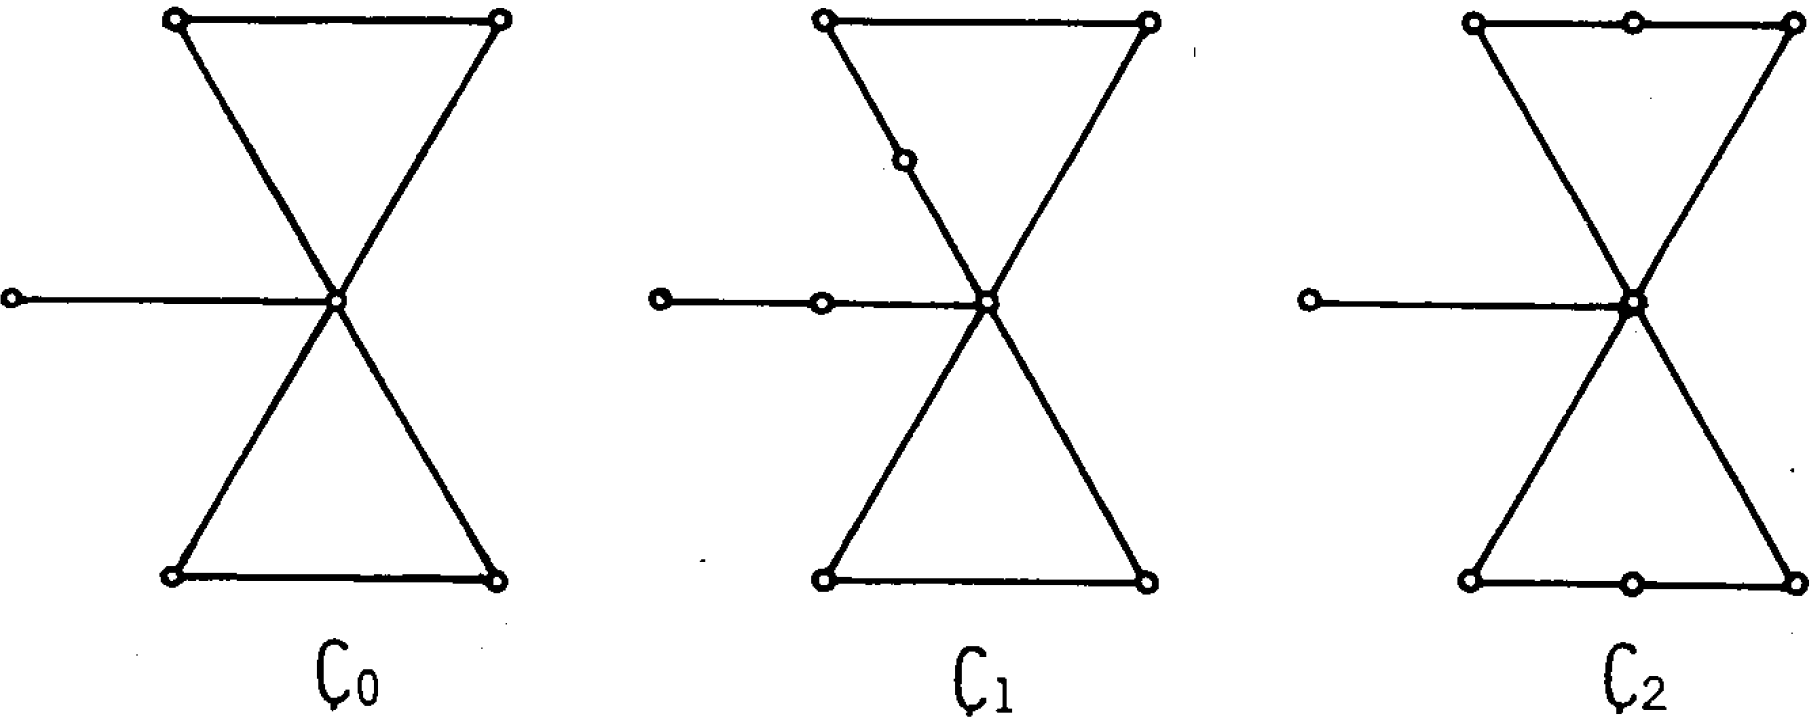
\includegraphics[width=0.85\textwidth]{images/ceyhun-188-fig01.png}
	\caption{Eşkökenli çizgeler.}
	\label{fig:Figure4.1.6}
\end{figure}

\end{document}